\chapter{Introduction.}
The time-series is a data type represented by a sequence of data points sampled at successive times and usually found as the sequence of real or integer numbers with attached timestamps. The time-series data is arising naturally from observations and reflecting an evolution of some subject or a development of some phenomena in time which makes time-series data ubiquitous and important not only in every scientific field but also in the everyday life. For example, it is very common to see in newspapers or on TV a visualized time-series representing financial information about stocks and currency fluctuations, weather changes or social trends. Medical observations such as a blood pressure, heart beat rate or a body temperature changes is another example of time-series commonly seen in life. According to Tufte \cite{citeulike:1454223} ``The time-series plot is the most frequently used form of graphic design. With one dimension marching along to the regular rhythm of seconds, minutes, hours, days, weeks, months, years, or millennia, the natural ordering of the time scale gives this design a strength and efficiency of interpretation found in no other graphic arrangement.'' The figure \ref{fig:10century} from the Tufte book depicts the oldest known example of a time-series plot showing the planetary orbits inclinations and is dated by tenth century.
\begin{figure}[tbp]
   \centering
   \includegraphics[height=70mm]{10century.eps}
   %%{seriesheatmap}
   \caption{Ancient time-series plot showing the planetary orbits inclinations.}
   \label{fig:10century}
\end{figure} 
It is generally assumed that the consecutive measured values in the time-series are sampled at equally spaced time intervals (which is not always true and if required, the resampling and interpolation used[citation needed]). This specific ordering of samples in time often bear the information about the dependency of successive observation on earlier ones and the explicit recognition of such ordering is a key feature which distinguishes the time-series data from usually independent statistical samples and makes the time-series analysis techniques somehow different from statistical analyses \cite{citeulike:3989988}. It should be noted, that while many time-series analyses methods treat time-series as the simple sequences of real numbers discarding the actual time-stamps, the time-ordering is always considered and it is assumed that unpronounced time interval are equal between the sampled values.

The time-series analysis methods in general combine various statistical and pattern recognition techniques while using information presented in the time-ordering of samples. Historically time-series analysis is divided by two major fields of study: first is the explorative and descriptive analysis and the second field is the forecasting. 
While the descriptive analyzes focused on the understanding of the time-series generating processes itself by finding trends, periodicity and some hidden features within the time-series [citation needed], the predictive analyses aiming forecasting the future of the time-series generating process based on the information found by conducting descriptive analyses \cite{citeulike:3449765}. 
Both, descriptive and predictive analyses, based on the identification of some pattern in the time-series which could be formally described and correspond to the time-series generating process nature. Once this pattern is found and compiled into the formal model during the explorative analysis it is used for the extrapolation of the time-series into future. Such a model development and forecasting could be traced from the babylonian astrologist predicting celestial phenomenas to the contemporary stochastic and deterministic models.

Taking in account the importance and value of time-series data and analyses, many of time-series databases were created for tracking various information. Contemporary trends in the cost of the data storage, increased bandwidth and progress in information science induced tremendous growth in the time series data volume and variety. There are public databases which tracking financial indexes and climate change (Figure \ref{fig:onlineDB}), astronomical observations \cite{citeulike:4373331} and medical information \cite{citeulike:4373332}. This tremendous growth in the data volume and availability during the last decade of the XX century demanded for new approaches in the KDD (Knowledge Discovery and Data mining) applications capable of handling of very large volumes of temporal data.
\begin{figure}[tbp]
   \centering
   \includegraphics[height=190mm]{onlineDB.eps}
   %%{seriesheatmap}
   \caption{Examples of time-series databases. Upper screenshot is the FRED (Federal Reserve Economic Data) database of 20,056 U.S. economic time series, lower is the part of the NOAA Climate time-series database.}
   \label{fig:onlineDB}
\end{figure} 
This literature review is focusing on the time-series similarity search algorithms which play a core role in many of the KDD applications such as clustering, classification , query by content, anomaly and motif detection. In particular, we will cover the basics of the time-series similarity measurements and major methods of the time-series dimensionality reduction used in the contemporarily state-of the art KDD applications following by their performance comparison based on the published results.